

\tikzset{every picture/.style={line width=0.75pt}} %set default line width to 0.75pt        

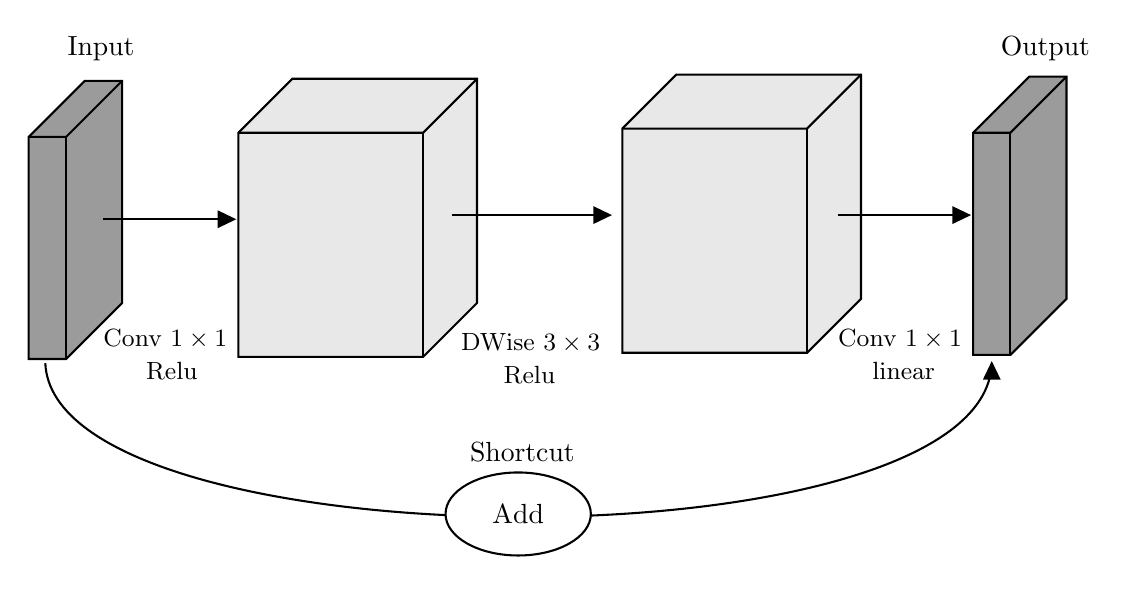
\begin{tikzpicture}[x=0.75pt,y=0.75pt,yscale=-1,xscale=1]
%uncomment if require: \path (0,600); %set diagram left start at 0, and has height of 600

%Shape: Cube [id:dp0950450187441989] 
\draw  [fill={rgb, 255:red, 155; green, 155; blue, 155 }  ,fill opacity=1 ] (24.17,60.33) -- (51.17,33.33) -- (69.17,33.33) -- (69.17,140.33) -- (42.17,167.33) -- (24.17,167.33) -- cycle ; \draw   (69.17,33.33) -- (42.17,60.33) -- (24.17,60.33) ; \draw   (42.17,60.33) -- (42.17,167.33) ;
%Shape: Cube [id:dp5388410753431343] 
\draw  [fill={rgb, 255:red, 155; green, 155; blue, 155 }  ,fill opacity=1 ] (479.17,58.33) -- (506.17,31.33) -- (524.17,31.33) -- (524.17,138.33) -- (497.17,165.33) -- (479.17,165.33) -- cycle ; \draw   (524.17,31.33) -- (497.17,58.33) -- (479.17,58.33) ; \draw   (497.17,58.33) -- (497.17,165.33) ;
%Shape: Cube [id:dp5352049268129733] 
\draw  [fill={rgb, 255:red, 232; green, 232; blue, 232 }  ,fill opacity=1 ] (125.17,58.33) -- (151.17,32.33) -- (240.17,32.33) -- (240.17,140.33) -- (214.17,166.33) -- (125.17,166.33) -- cycle ; \draw   (240.17,32.33) -- (214.17,58.33) -- (125.17,58.33) ; \draw   (214.17,58.33) -- (214.17,166.33) ;
%Shape: Cube [id:dp5972901431854747] 
\draw  [fill={rgb, 255:red, 232; green, 232; blue, 232 }  ,fill opacity=1 ] (310.17,56.33) -- (336.17,30.33) -- (425.17,30.33) -- (425.17,138.33) -- (399.17,164.33) -- (310.17,164.33) -- cycle ; \draw   (425.17,30.33) -- (399.17,56.33) -- (310.17,56.33) ; \draw   (399.17,56.33) -- (399.17,164.33) ;
%Curve Lines [id:da4213776555105224] 
\draw    (32.17,169.33) .. controls (36.15,266.84) and (483.66,269.31) .. (488.13,169.84) ;
\draw [shift={(488.17,168.33)}, rotate = 450] [fill={rgb, 255:red, 0; green, 0; blue, 0 }  ][line width=0.75]  [draw opacity=0] (8.93,-4.29) -- (0,0) -- (8.93,4.29) -- cycle    ;

%Straight Lines [id:da7525961556824932] 
\draw    (60,100) -- (122.17,100) ;
\draw [shift={(124.17,100)}, rotate = 180] [fill={rgb, 255:red, 0; green, 0; blue, 0 }  ][line width=0.75]  [draw opacity=0] (8.93,-4.29) -- (0,0) -- (8.93,4.29) -- cycle    ;

%Straight Lines [id:da7778926134720376] 
\draw    (228,98) -- (303.17,98) ;
\draw [shift={(305.17,98)}, rotate = 180] [fill={rgb, 255:red, 0; green, 0; blue, 0 }  ][line width=0.75]  [draw opacity=0] (8.93,-4.29) -- (0,0) -- (8.93,4.29) -- cycle    ;

%Straight Lines [id:da2814517292192529] 
\draw    (414,98) -- (476.17,98) ;
\draw [shift={(478.17,98)}, rotate = 180] [fill={rgb, 255:red, 0; green, 0; blue, 0 }  ][line width=0.75]  [draw opacity=0] (8.93,-4.29) -- (0,0) -- (8.93,4.29) -- cycle    ;

%Shape: Ellipse [id:dp8668947513316778] 
\draw  [fill={rgb, 255:red, 255; green, 255; blue, 255 }  ,fill opacity=1 ] (225,242) .. controls (225,230.95) and (240.67,222) .. (260,222) .. controls (279.33,222) and (295,230.95) .. (295,242) .. controls (295,253.05) and (279.33,262) .. (260,262) .. controls (240.67,262) and (225,253.05) .. (225,242) -- cycle ;

% Text Node
\draw (262,212) node  [align=left] {Shortcut};
% Text Node
\draw (90,165) node  [align=left] {{\small Conv $\displaystyle 1\times 1$}\\{\small  \ \ \ \ \ Relu}};
% Text Node
\draw (266,167) node  [align=left] {{\small DWise $\displaystyle 3\times 3$}\\{\small  \ \ \ \ \ Relu}};
% Text Node
\draw (444,165) node  [align=left] {{\small Conv $\displaystyle 1\times 1$}\\{\small  \ \ \ \ linear}};
% Text Node
\draw (260,242) node  [align=left] {Add};
% Text Node
\draw (59,18) node  [align=left] {Input};
% Text Node
\draw (514,18) node  [align=left] {Output};


\end{tikzpicture}